%%
%\listfiles
%\documentclass[%
% reprint,%
%secnumarabic,%
% amssymb, amsmath,%
% aip,cha,%
%groupedaddress,%
%frontmatterverbose,
%]{revtex4-1}
\documentclass[twocolumn,amsmath,amssymb,showpacs,pre,nofootinbib,superscriptaddress]{revtex4-1} %,preprint,jcp

\bibstyle{apsrev}
%\usepackage{docs}%
\usepackage{bm}%
\usepackage{graphicx}
%\usepackage{subcaption}
\usepackage{tikz}
\usepackage{color}
\usepackage{xcolor}
\usepackage{physics}
\usepackage[colorlinks=true,linkcolor=blue]{hyperref}%
%\nofiles
\expandafter\ifx\csname package@font\endcsname\relax\else
 \expandafter\expandafter
 \expandafter\usepackage
 \expandafter\expandafter
 \expandafter{\csname package@font\endcsname}%
\fi
\hyphenation{title}
\newcommand{\JH}[1]{\textcolor{blue}{ JH: #1}}

\begin{document}

\definecolor{pyblue}{HTML}{1F77B4}
\definecolor{pyorange}{HTML}{FF7F0C}
\definecolor{pygreen}{HTML}{2CA02C}
\definecolor{pyred}{HTML}{D62728}
\newcommand*\Diff[1]{\mathop{}\!\mathrm{d^#1}}


\title{Switchable substrates and thin film morphologies}

\author{S. Zitz}
\email{s.zitz@fz-juelich.de}
 \affiliation{Helmholtz Institute Erlangen-N\"urnberg for Renewable Energy,\\
  Forschungszentrum J\"ulich,\\
  F\"urther Strasse 248, 90429 N\"urnberg, Germany}%
  \affiliation{Department of Chemical and Biological Engineering, Friedrich-Alexander-Universit\"at Erlangen-N\"urnberg, F\"{u}rther Stra{\ss}e 248, 90429 N\"{u}rnberg, Germany}
\author{A. Scagliarini}%
\email{andrea.scagliarini@cnr.it}
 \affiliation{Institute for Applied Mathematics "M. Picone" (IAc, \\
Consiglio Nazionale delle Ricerche,\\
Via dei Taurini 19, 00185 Rome, Italy}%
\affiliation{INFN, sezione Roma ``Tor Vergata'', via della Ricerca Scientifica 1, 00133 Rome, Italy}
\author{J. Harting}
\email{j.harting@fz-juelich.de}
 \affiliation{Helmholtz Institute Erlangen-N\"urnberg for Renewable Energy,\\
  Forschungszentrum J\"ulich,\\
  F\"urther Strasse 248, 90429 N\"urnberg, Germany}%
 \affiliation{Department of Chemical and Biological Engineering and Department of Physics, Friedrich-Alexander-Universit\"at Erlangen-N\"urnberg, F\"{u}rther Stra{\ss}e 248, 90429 N\"{u}rnberg, Germany}
\date{\today}

\begin{abstract}
We study the dynamics of an unstable thin film deposited on a switchable substrate.
The substrate is itself subject to a time varying function that affects the equilibrium contact angle $\theta_{\text{eq}}(\mathbf{x},t)$.
We show that in the case of the vanishing time dependence the patterning drives the dewetting process and all fluid is drained into regions of a small $\theta_{\text{eq}}(\mathbf{x})$ and forms droplets.
Interestingly enough with a time varying equilibrium contact angle we are able to stop the droplet fragmentation and are able to create ligament or rivulet states.
We show that these rivulet states mainly depend on two quantities, first being the wavelength of the pattern and second being the velocity of the substrate pattern.

\end{abstract}

\maketitle

\newcommand{\ts}{\textsuperscript}
%\tableofcontents

\section{Introduction}\label{sec:intro}
Thin film flows and especially droplets are an phenomenon we experience in our every day life.
Rather unknown is the fact that our body uses thin films to cover mucous membranes.

\begin{equation}\label{eq:thin_film}
    \partial_t h(\mathbf{x},t) = \nabla\cdot\left(M(h)\nabla p(\mathbf{x},t)\right),
\end{equation}

\section{Method}\label{sec:method}
In this section we describe the lattice Boltzmann method (LBM) we use to simulate thin film flows.
The model we use has been introduced in ref~\cite{PhysRevE.100.033313} and builds upon a class of lattice Boltzmann models originally developed to study the shallow water equations~\cite{Salmon:1999:0022-2402:503, zhou2004lattice, PhysRevE.65.036309}.

\subsection{Thin film lattice Boltzmann method}\label{subsec:LBM}
The internal degrees of freedom of this method are the distributions functions $f_{\alpha}(\mathbf{x},t)$.
They describe a distribution of fictitious particles, for this paper we consider the case of $D2Q9$ lattice.
Such there are nine velocity components ($Q9$) for a simulation in two dimensions ($D2$).
The dynamics of the thin film and thus the evolution of the distribution functions is given by
\begin{equation}\label{eq:LBE}
    \begin{split}
        &f_{\alpha}(\mathbf{x}+\mathbf{c}^{({\alpha})}\Delta t,t+\Delta t) = \\
        &\left(1 - \frac{\Delta t}{\tau}\right) f_i(\mathbf{x},t) + \frac{\Delta t}{\tau} f_{\alpha}^{(eq)}(\mathbf{x},t) + \Delta t\mathcal{S}_{\alpha},
    \end{split}
\end{equation}
where the $\mathbf{c}^{({\alpha})}$ are the $Q$ discrete lattice velocities that can be computed according to
\begin{equation}\label{eq:speeds}
\mathbf{c}^{({\alpha})}  =
\left\{
\begin{array}{ll}
(0,0) & \alpha = 0 \\
\left[\cos{\frac{(\alpha-1)\pi}{4}}, \sin{\frac{(\alpha-1)\pi}{4}} \right] &  \alpha=1,3,5,7 \\
\sqrt{2}\left[\cos{\frac{(\alpha-1)\pi}{4}}, \sin{\frac{(\alpha-1)\pi}{4}} \right] & \alpha=2,4,6,8
\end{array}
\right.,
\end{equation}
and $w$ are being the corresponding weights
\begin{equation}
w_{\alpha}  =
\left\{
\begin{array}{ll}
\frac{4}{9} & \alpha = 0 \\
\frac{1}{9} &  \alpha=1,3,5,7 \\
\frac{1}{36} & \alpha=2,4,6,8
\end{array}
\right..
\end{equation}
The last term to the right $\mathcal{S}_{\alpha}$ is a (generalized) source term.
The concrete implementation of the forces depend on the source term as~\cite{https://doi.org/10.1002/fld.4726}
\begin{equation}\label{eq:source_term}
    \mathcal{S}_{\alpha} = \frac{3w_{\alpha}}{\mathbf{c}_{\alpha}^2}\mathbf{c}_{\alpha}\cdot\mathbf{F}.
\end{equation}
We are able to match thin film dynamics with the usage of a force term comprising of two main components,
\begin{equation}\label{eq:forcesum}
    \mathbf{F} = \mathbf{F}_{\mbox{\tiny{fric}}} + \mathbf{F}_{\mbox{\tiny{fric}}}.
\end{equation}
The first being a friction force that includes a velocity boundary condition at the fluid substrate interface
\begin{equation}\label{eq:forcefric}
\mathbf{F}_{\mbox{\tiny{fric}}} = -\frac{6h\mu\mathbf{u}}{2h^2+6\delta h + 3\delta^2},
\end{equation}
where $\mu$ is the viscosity and $\delta$ is a socalled slip length~\cite{RevModPhys.69.931, PhysRevE.100.033313, PhysRevE.63.011208, munch_lubrication_2005}.
The film thickness $h$ is the zeroth moment of the distribution function $f_{\alpha}$, i.e. $h(\mathbf{x},t) = \sum_{\alpha}f_{\alpha}(\mathbf{x},t)$ see Eq.~(\ref{eq:LBE}). 
The second component is due to the film pressure and accounts for the minimization of the fluid vapor interface as well as for the wettability of the substrate,
\begin{equation}\label{eq:forcefilm}
    \mathbf{F}_{\mbox{\tiny{film}}} = -\frac{\gamma h}{\rho_0}\nabla(\Delta h - \Pi(h)), 
\end{equation}
with $\gamma$ being the surface tension and $\rho_0$ being the fluids density, which is $\rho_0 = 1$ and will be dropped in the following. 
Here we model the interaction between solid substrate and film with a disjoining pressure term~\cite{RevModPhys.69.931, RevModPhys.81.1131, PhysRevE.63.011208},
\begin{equation}\label{eq:disjoinpressure}
    \Pi(h) = \kappa(\theta_{\text{eq.}})\left[\left(\frac{h_{\ast}}{h}\right)^n - \left(\frac{h_{\ast}}{h}\right)^m\right],
\end{equation}
with $n$ and $m$ being integer exponents, $h_{\ast}$ defines the minimum of the potential and  
\begin{equation}\label{eq:kappacontactangle}
    \kappa(\theta_{\text{eq.}}) = (1-\cos\theta_{\text{eq.}}) \frac{(n-1)(m-1)}{(n-m)h_{\ast}},
\end{equation}
which therefor allows us to tune the fluids contact angle.

\subsection{Linear stability and characteristic quantities}\label{subsec:charq}
For further insights concerning the early time dynamics of the unstable film we perform a linear stability analysis.
Thus we expand Eq.~(\ref{eq:thin_film}) in terms of a small perturbation $\delta h(\mathbf{x},t) = h(\mathbf{x},t) - h_0$ with $h_0$ being the initial mean thickness value at $t=0$.
Rearanging in terms up to first order in $\delta h$ yields
\begin{equation}\label{eq:linearstability_realspace}
    \partial_t \delta h = \frac{h_0^3}{3\mu}\nabla^2\Big(\Pi(\delta h) - \gamma \nabla^2 \delta h\Big).
\end{equation}
Under Fourier transformation of $\delta h$ 
\begin{equation}\label{eq:fouriertrans}
    \delta h(\mathbf{x},t) = \int(2\pi)^{-2}\delta \tilde{h}(\mathbf{q},t)e^{i\mathbf{q}\cdot\mathbf{x}}\Diff2\mathbf{q},
\end{equation}
and upon inserting this in Eq.~(\ref{eq:linearstability_realspace}) we get
\begin{equation}\label{eq:linearstab_fourier}
    \partial_t \delta \tilde{h}(\mathbf{q},t) = \omega(\mathbf{q})\delta\tilde{h}(\mathbf{q},t),
\end{equation}
with dispersion relation $\omega(q)$, 
\begin{equation}\label{eq:dispersion}
    \omega(\mathbf{q}) = \frac{1-(\frac{q^2}{q_0^2}-1)^2}{t_0}.
\end{equation}
Both, the maximum of the dispersion relation $q_0$ and therefore the characteristic time $t_0$, are specific to the substrate the film is deposited on and can be calculated using~\cite{PhysRevLett.99.114503}
\begin{equation}\label{eq:q0_and_t0}
    q_0^2 = \frac{1}{2}\frac{\partial \Pi(h)}{\partial h}\bigg\rvert_{h=h_0}, \qquad t_0 = \frac{3\mu}{\gamma h_0^3 q_0^4}.
\end{equation}

\subsection{Time and spatially varying contact angles $\theta(\mathbf{x},t)$}\label{subsec:theta}
To get a spatially varying contact angle $\theta(\mathbf{x},t)$ we make use of the underlying lattice and assign different values for $\theta$ to different grid points. 
From now on we drop the subscript \textit{eq.} for convenience, such $\theta = \theta_{\text{eq.}}$ unless otherwise stated.

We consider two different patterns and three wavelengths for this manuscript.
First being the sinusoidal pattern with wavelengths $\lambda \in \{L, L/2, L/3\}$ which is given as
\begin{equation}\label{eq:sinetheta}
    \theta_1(x,y) = \theta_0 + \delta\theta\left[\sin\left(\frac{2\pi x}{\lambda}\right)\sin\left(\frac{2\pi y}{\lambda}\right)\right], 
\end{equation}
with $\theta_0 = 20^{\circ}$ and $\delta\theta=10^{\circ}$.
The second pattern is a triangle wave which accounts for a more realistic szenario, thus $\theta_2$ is given as
\begin{equation}\label{eq:triangle_wave}
    \theta_2(x,y) = \theta_0 + \frac{2\delta\theta}{\pi}\left[\sin^{-1}\left(\sin\left(\frac{2\pi x}{\lambda}\right)\right)\sin^{-1}\left(\sin\left(\frac{2\pi y}{\lambda}\right)\right)\right].
\end{equation}

Both patterns create a contact angle distribution with values within the interval $[10^{\circ}, 30^{\circ}]$ and by definition they are time independent.
For a time dependent dynamic we simply shift the pattern in a periodic manner, such that
\begin{equation}\label{eq:theta_shift}
    \theta(\mathbf{x},t+T) = \theta(\mathbf{x}-\mathbf{1}, t), 
\end{equation}
with $T$ being an arbitrary number of lattice Boltzmann time steps. 

Due to convenience we artibute a velocity to the pattern which is simply the shift distance divided by the stepping time
\begin{equation}\label{eq:pattern_speed}
    v_{\theta} = \frac{\sqrt{2}}{T}.
\end{equation}
Since this velocity as well as the choice of $T$ is arbitrary we define a characteristic velocity $v_0$ similar to Eqs.~(\ref{eq:q0_and_t0}) as
\begin{equation}\label{eq:normvel}
    v_0 = \frac{\lambda}{t_0(\theta)},
\end{equation}
where we use the wavelength $\lambda$ as a characteristic distance and $t_0(30^{\circ})$ as a characteristic time scale.
Important to note is that $t_0$ is sensitive to the contact angle, and decreases with increasing angle.
Thus choosing the highest contact angle for the characteristic time scale means $t_0$ 

\subsection{Numerical system}
As outlined in Sec.~\ref{subsec:LBM} we simulate the evolution of the thin film with a lattice Boltzmann method.
For all our simulations we use periodic boundary conditions and a square of size $Lx = Ly = L = 512 \Delta x$ with $\Delta x = \Delta t = 1$.
The surface tension as well as the viscosity are constants and set to $\gamma = 0.01$ and $\mu = 1/6$.
Having this value of $\mu$ leaves us with a relaxation time $\tau = 1$.
To regularize the contact line divergence~\cite{huh1971hydrodynamic} we use a precursor layer and a slip length $\delta = 1$. 
With this choice of parameters we are almost able simulate a no-slip boundary condition.
As for our disjoining pressure potential, we use $n=3, m=2$ and $h_{\ast} = 0.07$.
Inserting this quantities into Eq.~(\ref{eq:q0_and_t0}) with $h_0 = 1$ yields $q_0^2(30^{\circ}) \approx 1.68\cdot10^{-2}$ as well as $t_0(30^{\circ}) \approx 177000\Delta t$ which gives us a first glimpse into relevant time scales.

The initial condition of all our simulations is a film undulated with sinusoidal wave as
\begin{equation}\label{eq:hinitial}
    h(\mathbf{x},0) = h_0 \left[1 + \epsilon \left(\sin\left(\frac{2\pi x}{L}\right)\sin\left(\frac{2\pi y}{L}\right)\right)\right],
\end{equation}
with $\epsilon = 0.1$ and $h_0 = 1$.

\section{Results}\label{sec:results}
\begin{figure}
    \centering
    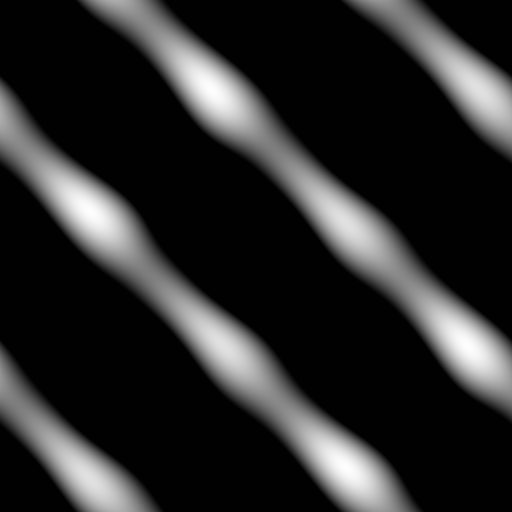
\includegraphics[width=0.45\textwidth]{Figures/theta_0336.png}
    \caption{Grayscale image of the height film at $t\approx 2t_0(30^{\circ})$}
    \label{fig:gray_ligament}
\end{figure}
We now present our results and show how a time dependent wettability or pattern velocity alters the morphology of the film during the dewetting process.
In the following we consider three time scales.
First being the initial short time behaviour that ends with the rupture of the film.
After the film ruptures we observe a transition region that strongly depend on the pattern velocity, see Fig.~\ref{fig:gray_ligament}.
Lastly we discuss the morphologies of the dewetted film in the long time regime.

\begin{figure}
    \centering
    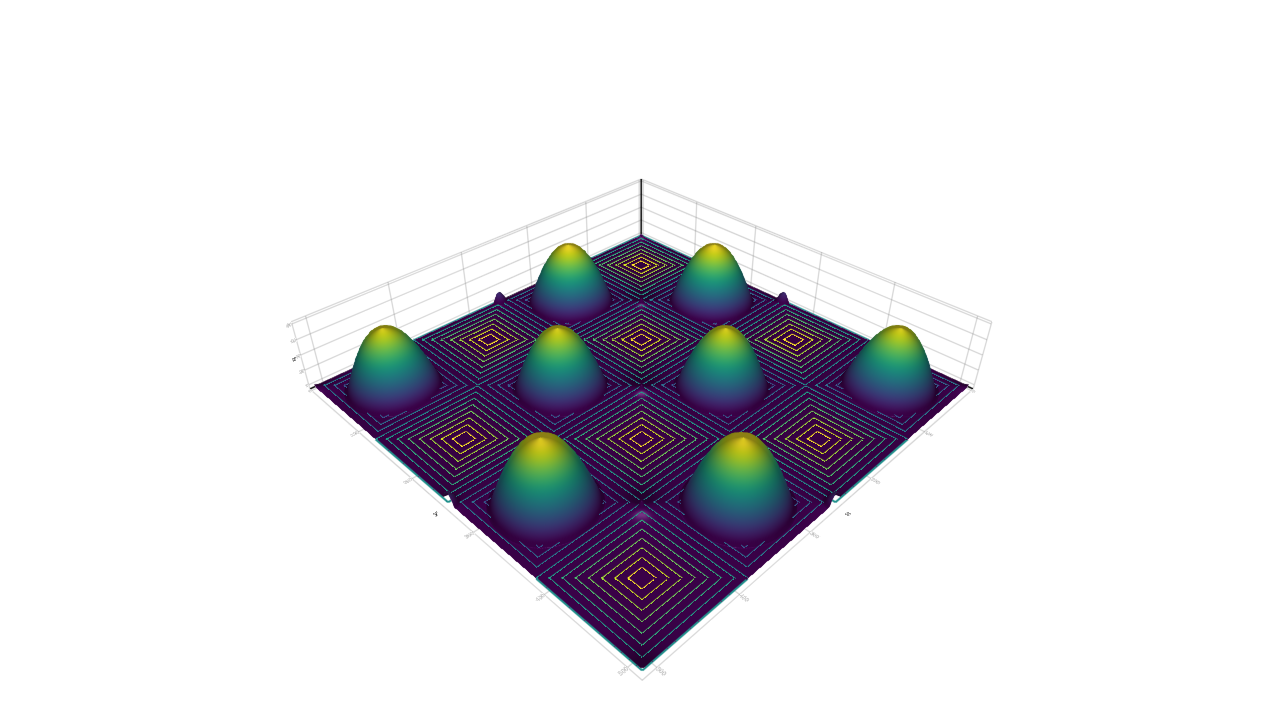
\includegraphics[width=0.45\textwidth]{Figures/makie_try2.png}
    \caption{Height of the film $h(\mathbf{x},t)$ with the contact angle $\theta(\mathbf{x})$ as contour.}
    \label{fig:handtheta}
\end{figure}
We proceed as follows, first we simulate the dewetting on a given pattern either sinusoidal- or triangular with $\lambda \in \{L, L/2, L/3\}$ without a time dependency in $\theta$.
In Fig.~\ref{fig:handtheta} we show $h(\mathbf{x},t)$ as surface plot and $\theta_2(\mathbf{x})$ as contour plot for $v_{\theta} = 0, \lambda = L/2$ in late stages of dewetting.
Subsequent simulations allow for $v_{\theta} \ne 0$.  
Based on $v_{\theta}$ we can modify the morphology of the dewetting film, in both the intermediate transition regime as well as the late time state.

\subsection{Early time behaviour}\label{subsec:earlyT}
Starting with Eq.~(\ref{eq:hinitial}) we have by definition an unstable film that will rupture.
Taking into account the addition of the wettability gradient we know that fluid will accumulate in regions of high surface energies or small contact angles.
This is shown in Fig.~\ref{fig:handtheta}, where all droplets are in a region of small contact angles.

\begin{figure*}
    \centering
    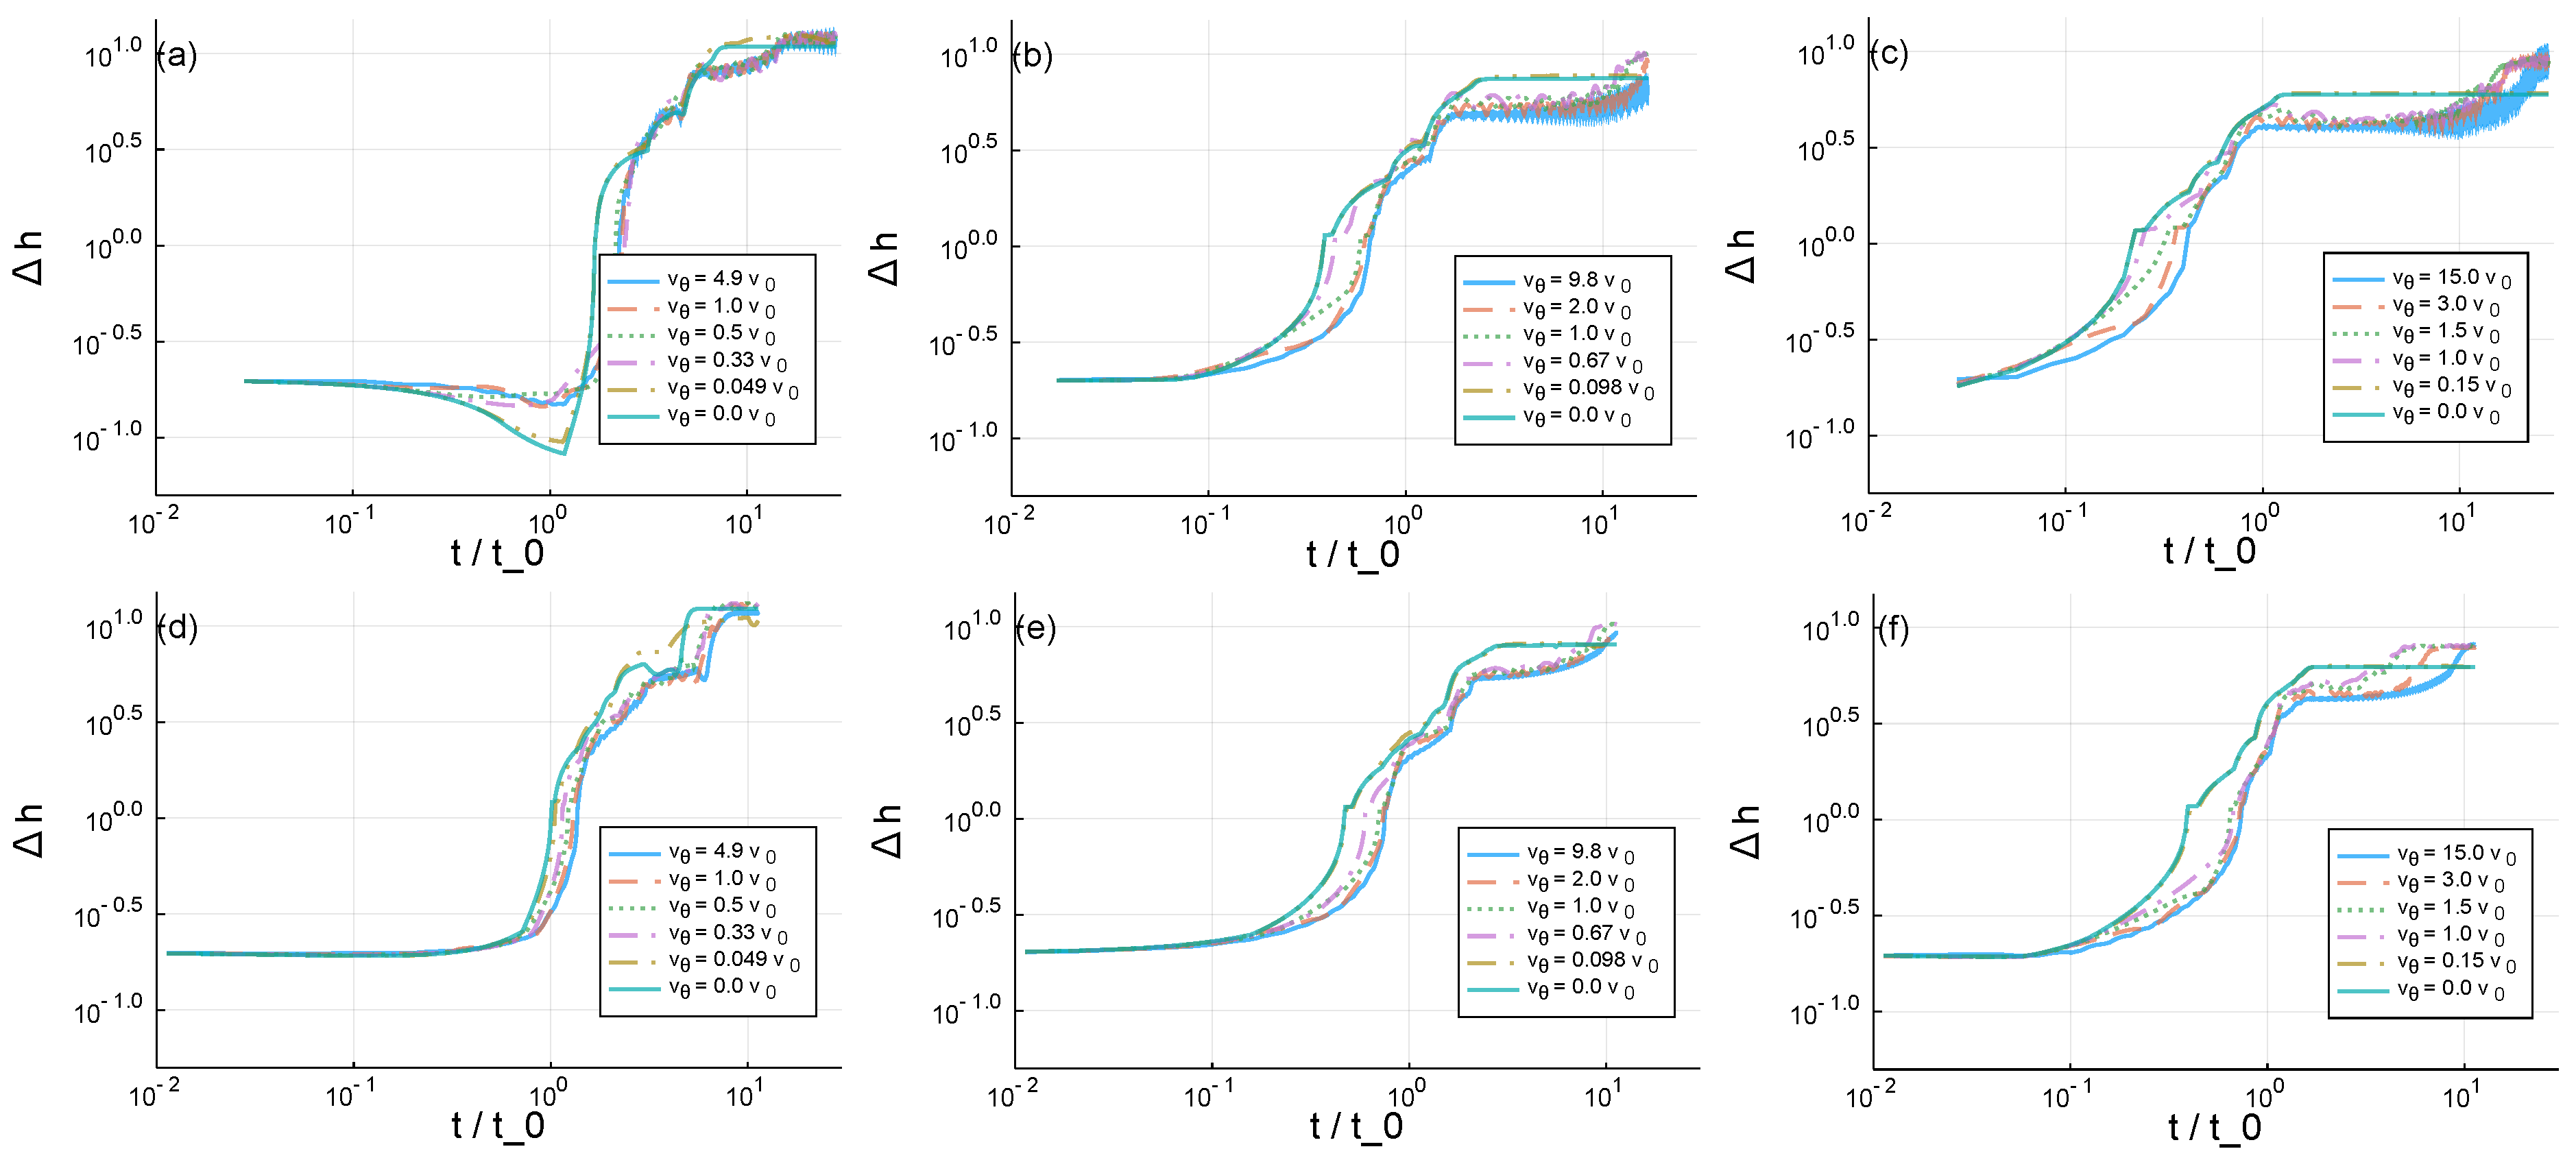
\includegraphics[width=\textwidth]{Figures/All_deltah.pdf}
    \caption{Evolution of the absolute difference in height, x-axis, up to $t\approx t_0(30^{\circ})$, y-axis, for different wavelengths and patterns.
    The upper series displays the data for $\theta_1$, see Eq.~(\ref{eq:sinetheta}), and $\lambda = L, L/2, L/3$ in (a,b,c) respectively.
    Below is the series for $\theta_2$, see Eq.~(\ref{eq:triangle_wave}).
    Different colors and line styles represent different pattern velocities, all of which are normalized with $v_0$, see Eq.~(\ref{eq:normvel}).}
    \label{fig:evolutin_deltah}
\end{figure*}
Naively one assumes in the early stages of the dewetting process that the perturbations grow exponentially~\cite{RevModPhys.69.931, RevModPhys.81.1131}.
This is not the case in our simulations as the initial conditions for $h$ as well as $\theta$ are the same, see Eq.~(\ref{eq:hinitial}, \ref{eq:sinetheta}).
We show this by measuring the time resolved difference between the maximum and the minimum of the height field as, 
\begin{equation}\label{eq:delta_h_measure}
    \Delta h(t) = \max_{\mathbf{x}}\{h(\mathbf{x},t)\} - \min_{\mathbf{x}}\{h(\mathbf{x},t)\},    
\end{equation}
which is shown in Fig.~\ref{fig:evolutin_deltah}.
In the upper row we show the data for $\theta_1$ while in the lower we show data for $\theta_2$, see Eqs.~(\ref{eq:sinetheta}-\ref{eq:triangle_wave}).
Different linestyles and colors represent different $v_{\theta}$'s.
Each column shows a wavelength $\lambda$, such from the left to the right we have $\lambda = L, L/2, L/3$.
Clearly one can observe the dip in \ref{fig:evolutin_deltah}(a) as the initial perturbation flattens while flowing into regions of lower contact angle.
This behaviour however is only pronounced for the time independent pattern and the smallest $v_{\theta}$ we use.
Thus the film is not spinodally dewetting but rather nucleating in regions of high contact angles.

Interestingly we observe a correlation between the rupture time ($\tau_r$) and the speed ($v_{\theta}$) as well as the wavelength ($\lambda$) of the pattern.
In agreement with previous studies on time dependent wettability we observe a stabilizing effect due to $v_{\theta}$~\cite{suman2006dynamics}.

\subsection{Intermediate times}\label{subsec:interT}
After the initial rupture of the film we observe that the dewetting is driven by $\theta(\mathbf{x},t)$.



\subsection{Long time behaviour}\label{subsec:lateT}

\section{Summary and Conclusions}\label{sec:sum_conclu}

\begin{acknowledgements}
The authors acknowledge financial support by the Deutsche Forschungsgemeinschaft (DFG) within the Cluster of Excellence ''Engineering of Advanced Materials'' (project EXC 315) (Bridge Funding). 
\end{acknowledgements}

%\appendix
%\section{}\label{app:one}

\bibliography{Ref}

\end{document}